\documentclass[12pt,a4paper]{report}

%--- Encodage & Langue ---
\usepackage[utf8]{inputenc}
\usepackage[T1]{fontenc}
\usepackage[french]{babel}

%--- Mise en page ---
\usepackage[top=2.5cm,bottom=2.5cm,left=3cm,right=2.5cm]{geometry}

%--- Graphiques & couleurs ---
\usepackage{graphicx}
\usepackage[dvipsnames,svgnames,x11names]{xcolor}
\usepackage{float}

%--- Tableaux ---
\usepackage{booktabs}
\usepackage{tabularx}
\usepackage{array}
\usepackage{colortbl}
\usepackage{tikz}
\usepackage{longtable}

%--- En-têtes & pieds de page ---
\usepackage{fancyhdr}

%--- Hyperliens ---
\usepackage[colorlinks=true,linkcolor=NavyBlue,urlcolor=RoyalBlue]{hyperref}

%--- Listes ---
\usepackage{enumitem}
\usepackage{pifont}

%--- Espacement ---
\usepackage{setspace}
\onehalfspacing

%--- Couleurs personnalisées ---
\definecolor{primary}{RGB}{0,71,171}
\definecolor{lightgray}{RGB}{245,245,245}
\definecolor{successgreen}{RGB}{34,139,34}

%--- En-têtes ---
\pagestyle{fancy}
\fancyhf{}
\fancyhead[L]{\small\textit{MecaManage}}
\fancyhead[R]{\small\textit{\leftmark}}
\fancyfoot[C]{\thepage}
\renewcommand{\headrulewidth}{0.4pt}

%=================================================================
\begin{document}
%=================================================================

%--- PAGE DE TITRE ---
\begin{titlepage}
\newcommand{\HRule}{\rule{\linewidth}{0.5mm}}
\centering

\begin{minipage}[l]{0.15\textwidth}
  
\includegraphics[width=3.5cm,height=2cm]{tekup.png}
\end{minipage}
\hfill
\begin{minipage}[c]{0.60\textwidth}
  \centering
  \footnotesize
  \textbf{\textsc{R\'{e}publique tunisienne}}\\[2pt]
  \textbf{\textsc{Minist\`{e}re de l'Enseignement sup\'{e}rieur
    et de la Recherche scientifique}}\\[4pt]
  \textbf{\textsc{TEK-UP University}}\\[4pt]
  \textbf{\textsc{\'{E}cole priv\'{e}e sup\'{e}rieure
    de technologie et d'ing\'{e}nierie}}
\end{minipage}
\hfill
\begin{minipage}[r]{0.15\textwidth}
  \hfill
\end{minipage}

\vskip1cm

\textsc{\huge Conception et Impl\'{e}mentation d'un Syst\`{e}me
  Intelligent\\[0.3cm] de Gestion d'Atelier Automobile}\\[0.5cm]

\textbf{\large Pr\'{e}sent\'{e} en vue de l'obtention de la}\\[0.5cm]
\textsc{\large Cycle d'Ing\'{e}nieur en Informatique}\\[0.5cm]
\textbf{Parcours~: G\'{e}nie Logiciel}\\[0.3cm]

\vskip1cm
\textit{R\'{e}alis\'{e} par}\\[0.5cm]
\textsc{\large Ihebeddine Saafi \quad|\quad Arbi Hazbri
  \quad|\quad Louay Lewati}\\[0.5cm]

\HRule\\[0.2cm]
{\textcolor{primary}{\LARGE\bfseries MecaManage}}\\[0.3cm]
\HRule\\[1cm]

{Th\`{e}me du projet}\\[0.2cm]

\includegraphics[width=0.4\textwidth]{mm.png}\\

\vskip1cm
{\large Ann\'{e}e Universitaire~: 2025--2026}

\vfill
\end{titlepage}

%=================================================================
% TABLE DES MATIÈRES
%=================================================================
\tableofcontents
\listoffigures
\newpage

%=================================================================
% INTRODUCTION GÉNÉRALE
%=================================================================
\chapter*{Introduction G\'{e}n\'{e}rale}
\addcontentsline{toc}{chapter}{Introduction G\'{e}n\'{e}rale}
\markboth{Introduction G\'{e}n\'{e}rale}{}

\section*{Contexte et Motivation}

L'industrie automobile conna\^{i}t une transformation profonde port\'{e}e
par la num\'{e}risation des processus m\'{e}tiers, la mont\'{e}e en puissance
de l'intelligence artificielle et l'exigence croissante de qualit\'{e} de
service de la part des clients. Les garages et ateliers m\'{e}caniques font
face \`{a} des d\'{e}fis op\'{e}rationnels majeurs~: gestion inefficace des
rendez-vous, suivi manuel des r\'{e}parations, absence de tra\c{c}abilit\'{e}
des stocks et difficult\'{e} \`{a} exploiter les donn\'{e}es historiques.

\medskip

La majorit\'{e} des solutions existantes sur le march\'{e} restent soit trop
g\'{e}n\'{e}riques, soit trop rudimentaires pour r\'{e}pondre aux besoins
d'entreprises multi-\'{e}tablissements. C'est dans cette perspective que
s'inscrit le projet \textbf{MecaManage}~: une plateforme SaaS
(\textit{Software as a Service}) de gestion d'ateliers m\'{e}caniques
con\c{c}ue pour les entreprises exploitant plusieurs garages.

\section*{Probl\'{e}matique}

Les entreprises de garages multi-\'{e}tablissements sont confront\'{e}es
\`{a} plusieurs probl\`{e}mes r\'{e}currents~:

\begin{itemize}[leftmargin=1.5cm]
  \item \textbf{Fragmentation des donn\'{e}es}~: chaque garage g\`{e}re
    son propre stock et ses plannings sans vision consolid\'{e}e.
  \item \textbf{Absence d'intelligence diagnostique}~: le diagnostic repose
    enti\`{e}rement sur l'expertise humaine sans capitalisation.
  \item \textbf{Manque de tra\c{c}abilit\'{e}}~: le suivi des r\'{e}parations
    n'est pas accessible en temps r\'{e}el aux clients.
  \item \textbf{Processus manuels co\^{u}teux}~: devis, notifications et
    relances sont trait\'{e}s manuellement.
  \item \textbf{Absence de reporting consolid\'{e}}~: pas de tableau de bord
    agr\'{e}g\'{e} multi-garage.
\end{itemize}

\section*{Objectifs du Projet}

\begin{enumerate}[leftmargin=1.5cm]
  \item Fournir une \textbf{plateforme SaaS multi-tenant} pour la gestion
    centralis\'{e}e de plusieurs garages.
  \item Int\'{e}grer un \textbf{module de diagnostic assist\'{e} par IA}
    pour l'analyse des sympt\^{o}mes.
  \item Automatiser les \textbf{workflows m\'{e}tiers} via n8n.
  \item Offrir un \textbf{suivi en temps r\'{e}el} des interventions.
  \item Mettre en place une \textbf{infrastructure DevOps industrialis\'{e}e}
    garantissant disponibilit\'{e}, s\'{e}curit\'{e} et scalabilit\'{e}.
\end{enumerate}

\section*{Structure du Rapport}

\begin{description}[leftmargin=2cm]
  \item[\textbf{Chapitre~1}] \'{E}tude pr\'{e}alable et sp\'{e}cification
    des besoins~: analyse de l'existant, acteurs, UML, architecture.
  \item[\textbf{Chapitre~2}] Conception d\'{e}taill\'{e}e~: microservices,
    mod\'{e}lisation des donn\'{e}es, interfaces.
  \item[\textbf{Chapitre~3}] Impl\'{e}mentation~: ASP.NET Core~8,
    Angular~17, Python FastAPI.
  \item[\textbf{Chapitre~4}] Infrastructure et DevOps~: Docker, CI/CD,
    Ansible, monitoring.
  \item[\textbf{Conclusion}] Bilan, limites et perspectives.
\end{description}

\newpage

%=================================================================
% CHAPITRE 1
%=================================================================
\chapter{\'{E}tude Pr\'{e}alable et Sp\'{e}cification des Besoins}

\section*{Introduction}
Ce premier chapitre pose les fondations du projet MecaManage.
Apr\`{e}s une analyse de l'existant et une identification des besoins,
nous pr\'{e}sentons les acteurs, les cas d'utilisation, le diagramme
de classes et l'architecture technique retenue.

%--- 1.1 ---
\section{Analyse de l'Existant}

\subsection{Solutions Actuelles sur le March\'{e}}

\begin{table}[H]
\centering
\caption{Comparaison des solutions existantes}
\label{tab:comparaison}
\renewcommand{\arraystretch}{1.3}
\begin{tabularx}{\textwidth}{|l|X|X|X|}
\hline
\rowcolor{primary!20}
\textbf{Crit\`{e}re} & \textbf{Solutions g\'{e}n\'{e}riques}
  & \textbf{ERP automobiles} & \textbf{MecaManage} \\
\hline
Multi-\'{e}tablissements & Limit\'{e} & Partiel
  & \textcolor{successgreen}{\ding{51}} Complet \\
\hline
Diagnostic IA & \textcolor{red}{\ding{55}} & \textcolor{red}{\ding{55}}
  & \textcolor{successgreen}{\ding{51}} Int\'{e}gr\'{e} \\
\hline
SaaS natif & Rare & Non
  & \textcolor{successgreen}{\ding{51}} Natif \\
\hline
Automatisation workflows & \textcolor{red}{\ding{55}} & Partiel
  & \textcolor{successgreen}{\ding{51}} n8n \\
\hline
Suivi temps r\'{e}el & \textcolor{red}{\ding{55}} & \textcolor{red}{\ding{55}}
  & \textcolor{successgreen}{\ding{51}} Inclus \\
\hline
DevOps / Open API & \textcolor{red}{\ding{55}} & \textcolor{red}{\ding{55}}
  & \textcolor{successgreen}{\ding{51}} Docker + CI/CD \\
\hline
\end{tabularx}
\end{table}

\subsection{Limites Identifi\'{e}es}

\begin{itemize}
  \item Absence de capitalisation sur les donn\'{e}es historiques de
    r\'{e}paration pour alimenter un module de diagnostic automatis\'{e}.
  \item Architecture monolithique incompatible avec des d\'{e}ploiements
    SaaS multi-tenant.
  \item Pas d'API ouverte permettant l'int\'{e}gration avec des outils
    tiers (n8n, Prometheus, etc.).
  \item Interface client rudimentaire, sans portail de suivi en temps r\'{e}el.
\end{itemize}

%--- 1.2 ---
\section{Identification des Acteurs}

\begin{table}[H]
\centering
\caption{Acteurs du syst\`{e}me MecaManage}
\label{tab:acteurs}
\renewcommand{\arraystretch}{1.4}
\begin{tabularx}{\textwidth}{|l|X|l|}
\hline
\rowcolor{primary!20}
\textbf{Acteur} & \textbf{R\^{o}le} & \textbf{Port\'{e}e} \\
\hline
\textbf{SuperAdmin} & Gestion globale de la plateforme SaaS, tenants
  & Plateforme \\
\hline
\textbf{Admin Entreprise} & Gestion garages, reporting, configuration
  & Entreprise \\
\hline
\textbf{Chef d'Atelier} & Dossiers, affectation m\'{e}caniciens, devis
  & Garage \\
\hline
\textbf{M\'{e}canicien} & Ex\'{e}cution des interventions assign\'{e}es
  & Garage \\
\hline
\textbf{Client} & Demandes, suivi r\'{e}parations en temps r\'{e}el
  & Portail client \\
\hline
\end{tabularx}
\end{table}

%--- 1.3 ---
\section{Sp\'{e}cification des Besoins}

\subsection{Besoins Fonctionnels}

\subsubsection{Module Gestion Clients et V\'{e}hicules}
\begin{itemize}
  \item Cr\'{e}ation et authentification des comptes clients
    (JWT + Refresh Tokens).
  \item Enregistrement des v\'{e}hicules avec historique complet.
  \item Soumission de demandes via formulaire intelligent
    (photos, kilom\'{e}trage, description libre des sympt\^{o}mes).
\end{itemize}

\subsubsection{Module Diagnostic IA}
\begin{itemize}
  \item Analyse NLP des sympt\^{o}mes d\'{e}crits en langage naturel.
  \item Production d'un diagnostic probable avec score de confiance.
  \item Recommandation du type d'atelier requis
    (m\'{e}canique, \'{e}lectrique, hybride).
\end{itemize}

\subsubsection{Module Gestion des Interventions}
\begin{itemize}
  \item Affectation des dossiers par l'admin aux chefs d'atelier.
  \item Acceptation / refus avec notification automatique client.
  \item Suivi du statut en temps r\'{e}el~:
    \textit{En attente $\rightarrow$ Accept\'{e} $\rightarrow$ En cours
    $\rightarrow$ En attente pi\`{e}ces $\rightarrow$ Termin\'{e}}.
  \item G\'{e}n\'{e}ration de devis dynamiques en cas de remplacement
    de pi\`{e}ces.
\end{itemize}

\subsubsection{Module Stock}
\begin{itemize}
  \item Gestion du stock par \'{e}tablissement avec tra\c{c}abilit\'{e}.
  \item R\'{e}servation automatique des pi\`{e}ces lors de l'acceptation
    d'un devis.
  \item Alertes de stock minimum via n8n.
\end{itemize}

\subsubsection{Module Facturation et Reporting}
\begin{itemize}
  \item G\'{e}n\'{e}ration automatique des factures en fin d'intervention.
  \item Tableau de bord Admin~: CA global, performance par garage,
    taux d'acceptation devis, rendement m\'{e}caniciens.
\end{itemize}

\subsection{Besoins Non Fonctionnels}

\begin{table}[H]
\centering
\caption{Besoins non fonctionnels}
\renewcommand{\arraystretch}{1.3}
\begin{tabularx}{\textwidth}{|l|X|}
\hline
\rowcolor{primary!20}
\textbf{Cat\'{e}gorie} & \textbf{Exigence} \\
\hline
Performance & Temps de r\'{e}ponse API $<200$\,ms (p95),
  500 utilisateurs simultan\'{e}s \\
\hline
Disponibilit\'{e} & SLA 99,9\,\% --- d\'{e}ploiement z\'{e}ro-downtime
  via Ansible \\
\hline
S\'{e}curit\'{e} & HTTPS TLS~1.3, JWT, isolation r\'{e}seau Docker,
  Rate Limiting \\
\hline
Scalabilit\'{e} & Architecture microservices horizontalement scalable \\
\hline
RGPD & Droit \`{a} l'effacement, export donn\'{e}es, consentements \\
\hline
Maintenabilit\'{e} & Clean Architecture, couverture tests $>80$\,\%,
  docs OpenAPI \\
\hline
\end{tabularx}
\end{table}

%--- 1.4 ---
\section{Diagramme de Cas d'Utilisation}

Le diagramme de cas d'utilisation global
(Figure~\ref{fig:uc_global}) repr\'{e}sente les interactions entre
les cinq acteurs et les principaux cas d'utilisation du syst\`{e}me.

\begin{figure}[H]
  \centering
  
\includegraphics[width=0.40\textwidth]{uc_global.png}
  \caption{Diagramme de cas d'utilisation global --- MecaManage}
  \label{fig:uc_global}
\end{figure}

\subsection{Description des Cas d'Utilisation Principaux}

\subsubsection{UC01 --- S'inscrire et S\'{e}lectionner un Garage}

\begin{table}[H]
\centering
\caption{Fiche UC01 --- S'inscrire et s\'{e}lectionner un garage}
\renewcommand{\arraystretch}{1.3}
\begin{tabularx}{\textwidth}{|l|X|}
\hline
\rowcolor{lightgray}
\textbf{Champ} & \textbf{Description} \\
\hline
Acteur principal & Client \\
\hline
Pr\'{e}condition & Aucune \\
\hline
Sc\'{e}nario nominal &
  1. Le client acc\`{e}de au portail et cr\'{e}e son compte. \newline
  2. Le syst\`{e}me d\'{e}tecte sa localisation g\'{e}ographique. \newline
  3. Le client visualise les garages disponibles. \newline
  4. Il s\'{e}lectionne un garage selon la distance ou la
     disponibilit\'{e}. \\
\hline
Postcondition & Compte cr\'{e}\'{e}, garage s\'{e}lectionn\'{e},
  session ouverte. \\
\hline
Exceptions & Aucun garage disponible $\rightarrow$ cr\'{e}neau
  ult\'{e}rieur propos\'{e}. \\
\hline
\end{tabularx}
\end{table}

\subsubsection{UC02 --- Soumettre une Demande d'Intervention}

\begin{table}[H]
\centering
\caption{Fiche UC02 --- Soumettre une demande d'intervention}
\renewcommand{\arraystretch}{1.3}
\begin{tabularx}{\textwidth}{|l|X|}
\hline
\rowcolor{lightgray}
\textbf{Champ} & \textbf{Description} \\
\hline
Acteur principal & Client \\
\hline
Pr\'{e}condition & Client authentifi\'{e}, garage s\'{e}lectionn\'{e}. \\
\hline
Sc\'{e}nario nominal &
  1. Le client remplit le formulaire (v\'{e}hicule, km, photos,
     sympt\^{o}mes). \newline
  2. Il soumet la demande. \newline
  3. Le microservice IA analyse les sympt\^{o}mes (\texttt{<<include>>}).
     \newline
  4. Un diagnostic probable est attach\'{e} au dossier. \newline
  5. L'administrateur est notifi\'{e} automatiquement. \\
\hline
Postcondition & Dossier cr\'{e}\'{e} avec diagnostic IA, admin notifi\'{e}. \\
\hline
Extensions & \texttt{<<include>>} Analyser sympt\^{o}mes par IA. \\
\hline
\end{tabularx}
\end{table}

\subsubsection{UC03 --- G\'{e}rer les Dossiers (Chef d'Atelier)}

\begin{table}[H]
\centering
\caption{Fiche UC03 --- G\'{e}rer les dossiers}
\renewcommand{\arraystretch}{1.3}
\begin{tabularx}{\textwidth}{|l|X|}
\hline
\rowcolor{lightgray}
\textbf{Champ} & \textbf{Description} \\
\hline
Acteur principal & Chef d'Atelier \\
\hline
Pr\'{e}condition & Dossier affect\'{e} par l'admin. \\
\hline
Sc\'{e}nario nominal &
  1. Le chef d'atelier consulte le dossier et le diagnostic IA. \newline
  2. Il accepte ou refuse le dossier. \newline
  3. Si accept\'{e}~: date fix\'{e}e, client notifi\'{e}
     (email + SMS). \newline
  4. Si pi\`{e}ces n\'{e}cessaires~: devis g\'{e}n\'{e}r\'{e} et
     envoy\'{e} au client. \newline
  5. Fin d'intervention~: facture g\'{e}n\'{e}r\'{e}e automatiquement. \\
\hline
Postcondition & Client notifi\'{e}, workflow mis \`{a} jour. \\
\hline
Extensions & \texttt{<<extend>>} G\'{e}n\'{e}rer devis si pi\`{e}ces
  n\'{e}cessaires. \\
\hline
\end{tabularx}
\end{table}

%--- 1.5 ---
\section{Diagramme de Classes}

Le diagramme de classes (Figure~\ref{fig:class_diagram}) mod\'{e}lise
les entit\'{e}s principales du domaine m\'{e}tier et leurs relations,
suivant les principes de la Clean Architecture.

\begin{figure}[H]
  \centering
  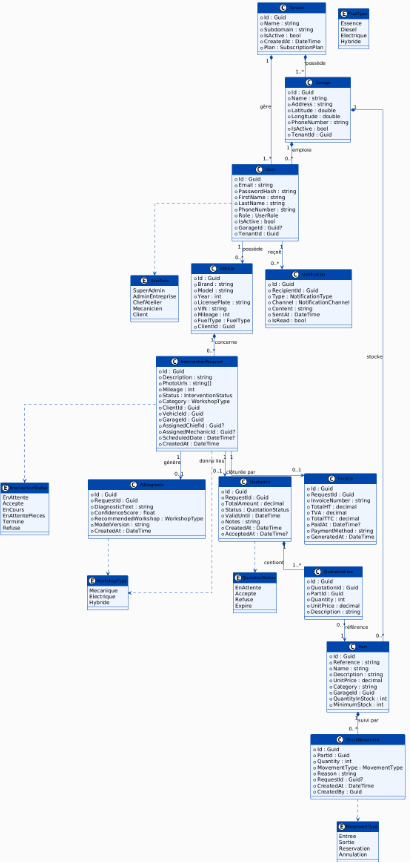
\includegraphics[width=\textwidth]{class_diagram.png}
  \caption{Diagramme de classes --- Domaine MecaManage}
  \label{fig:class_diagram}
\end{figure}

\subsection{Description des Entit\'{e}s Principales}

\begin{description}[leftmargin=1.5cm]
  \item[\textbf{Tenant}] Entreprise cliente de la plateforme SaaS.
    Chaque tenant poss\`{e}de un ou plusieurs garages.
  \item[\textbf{Garage}] \'{E}tablissement physique avec son propre stock,
    ses chefs d'atelier et ses m\'{e}caniciens.
  \item[\textbf{User}] Entit\'{e} de base~: SuperAdmin, AdminEntreprise,
    ChefAtelier, M\'{e}canicien, Client.
  \item[\textbf{Vehicle}] V\'{e}hicule associ\'{e} \`{a} un client avec
    historique complet.
  \item[\textbf{InterventionRequest}] Demande d'intervention incluant
    le diagnostic IA et le statut courant.
  \item[\textbf{AIDiagnosis}] R\'{e}sultat IA~: diagnostic textuel,
    score de confiance, type d'atelier recommand\'{e}.
  \item[\textbf{Quotation}] Devis g\'{e}n\'{e}r\'{e} par le chef d'atelier
    pour une intervention n\'{e}cessitant des pi\`{e}ces.
  \item[\textbf{Invoice}] Facture finale g\'{e}n\'{e}r\'{e}e
    automatiquement \`{a} la cl\^{o}ture.
  \item[\textbf{Part}] Pi\`{e}ce de rechange dans le stock d'un garage.
  \item[\textbf{StockMovement}] Tra\c{c}abilit\'{e} des mouvements de
    stock (entr\'{e}e / sortie / r\'{e}servation).
\end{description}

%--- 1.6 ---
\section{Architecture du Syst\`{e}me}

\subsection{Vue d'Ensemble --- Architecture Microservices}

MecaManage adopte une architecture microservices conteneuris\'{e}e
(Figure~\ref{fig:architecture}) garantissant la scalabilit\'{e}
horizontale, l'isolation des composants et la r\'{e}silience.

\begin{figure}[H]
  \centering
  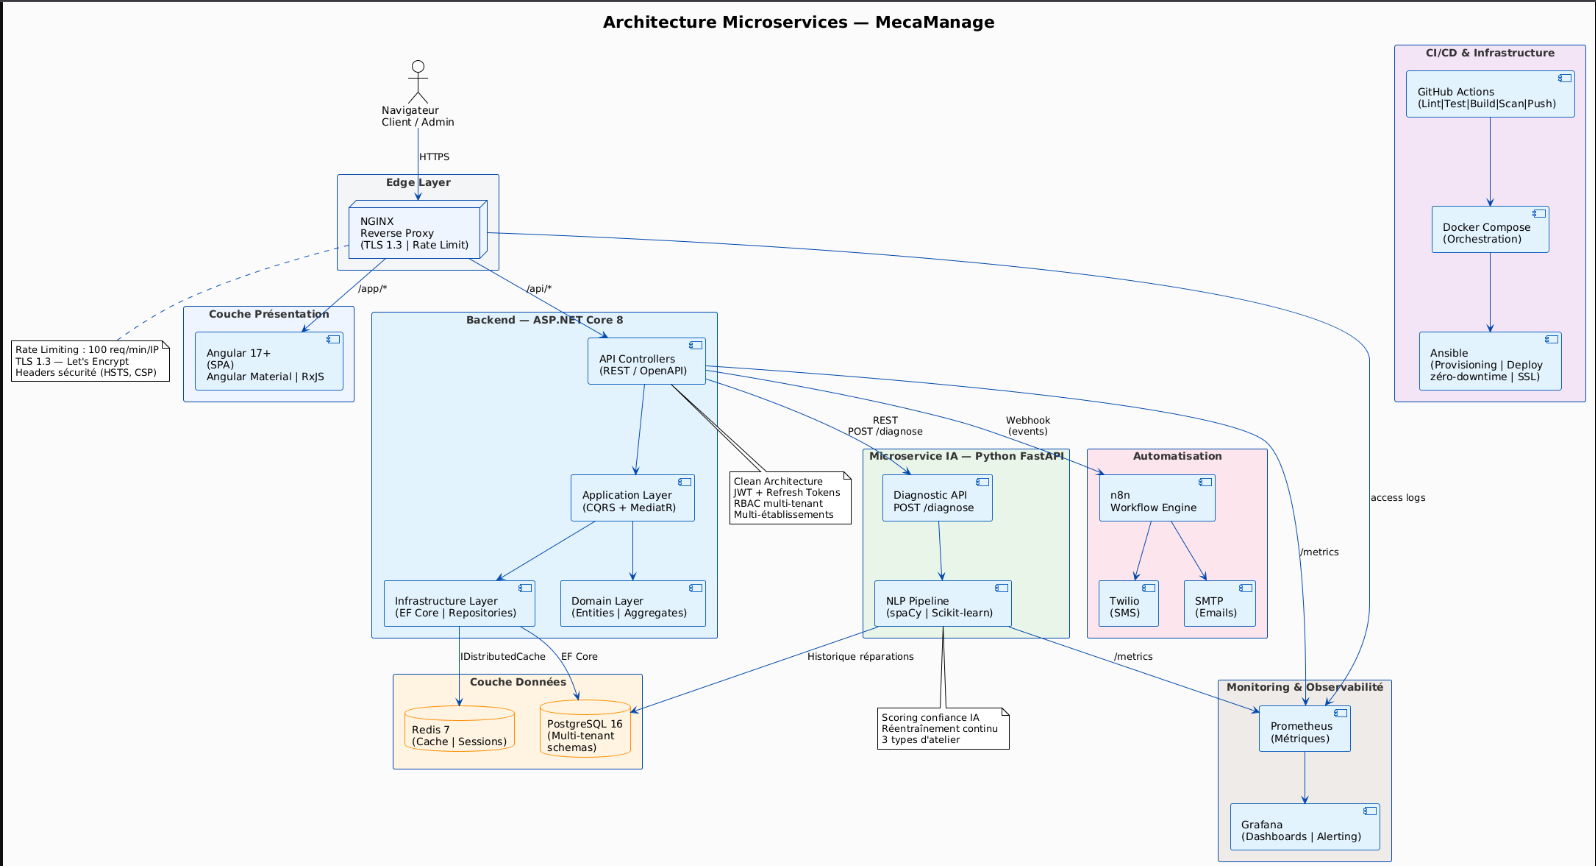
\includegraphics[width=\textwidth]{architecture.png}
  \caption{Architecture microservices --- MecaManage}
  \label{fig:architecture}
\end{figure}

\subsection{Composants de l'Architecture}

\subsubsection{Couche Pr\'{e}sentation}
\begin{itemize}
  \item \textbf{Angular~17+} avec Angular Material et RxJS ---
    interface client et portail d'administration (SPA).
  \item D\'{e}ploy\'{e} via un conteneur NGINX servant les assets
    statiques compil\'{e}s.
\end{itemize}

\subsubsection{API Gateway --- NGINX Reverse Proxy}
\begin{itemize}
  \item Routage des requ\^{e}tes vers les microservices appropri\'{e}s.
  \item Terminaison TLS~1.3, Rate Limiting, compression gzip.
\end{itemize}

\subsubsection{Backend Principal --- ASP.NET Core~8}
\begin{itemize}
  \item \textbf{Clean Architecture}~: Domain / Application /
    Infrastructure / API.
  \item Pattern \textbf{CQRS + MediatR} pour la s\'{e}paration des
    commandes et des requ\^{e}tes.
  \item \textbf{Entity Framework Core} avec PostgreSQL~16.
  \item Authentification \textbf{JWT + Refresh Tokens}, RBAC
    multi-r\^{o}les et multi-tenant.
  \item Cache \textbf{Redis~7} pour sessions et donn\'{e}es
    fr\'{e}quemment acc\'{e}d\'{e}es.
\end{itemize}

\subsubsection{Microservice IA --- Python FastAPI}
\begin{itemize}
  \item API REST pour l'analyse des sympt\^{o}mes en langage naturel.
  \item Pipeline NLP~: pr\'{e}traitement $\rightarrow$ vectorisation
    $\rightarrow$ classification (Scikit-learn + spaCy).
  \item R\'{e}entra\^{i}nement continu \`{a} partir des donn\'{e}es
    valid\'{e}es par les chefs d'atelier.
\end{itemize}

\subsubsection{Automatisation --- n8n}
\begin{itemize}
  \item Rappels RDV, notifications acceptation/refus, relances devis,
    alertes stock, rapports hebdomadaires.
  \item Int\'{e}gration SMTP, Twilio (SMS), webhooks API principale.
\end{itemize}

\subsubsection{Infrastructure DevOps}
\begin{itemize}
  \item \textbf{Docker + Docker Compose} pour l'orchestration.
  \item \textbf{GitHub Actions}~: lint $\rightarrow$ tests
    $\rightarrow$ build $\rightarrow$ scan s\'{e}curit\'{e}
    $\rightarrow$ push registry $\rightarrow$ d\'{e}ploiement.
  \item \textbf{Ansible}~: provisioning, d\'{e}ploiement
    z\'{e}ro-downtime, SSL Let's Encrypt.
  \item \textbf{Prometheus + Grafana}~: monitoring, alerting,
    dashboards.
\end{itemize}

\subsection{Stack Technique R\'{e}capitulatif}

\begin{table}[H]
\centering
\caption{Stack technique MecaManage}
\renewcommand{\arraystretch}{1.3}
\begin{tabularx}{\textwidth}{|l|l|X|}
\hline
\rowcolor{primary!20}
\textbf{Couche} & \textbf{Technologie} & \textbf{R\^{o}le} \\
\hline
Frontend & Angular~17 + Material & Interface utilisateur SPA \\
\hline
Backend & ASP.NET Core~8 & API REST, logique m\'{e}tier, CQRS \\
\hline
Base de donn\'{e}es & PostgreSQL~16 & Persistance relationnelle \\
\hline
Cache & Redis~7 & Sessions, cache applicatif \\
\hline
IA & Python FastAPI + Scikit-learn & Diagnostic automatis\'{e} NLP \\
\hline
Automatisation & n8n & Workflows m\'{e}tiers automatis\'{e}s \\
\hline
Reverse Proxy & NGINX & Routage, TLS, rate limiting \\
\hline
Conteneurisation & Docker + Compose & Isolation et portabilit\'{e} \\
\hline
CI/CD & GitHub Actions & Int\'{e}gration et d\'{e}ploiement continus \\
\hline
IaC & Ansible & Provisioning et d\'{e}ploiement \\
\hline
Monitoring & Prometheus + Grafana & Observabilit\'{e} syst\`{e}me \\
\hline
\end{tabularx}
\end{table}

%--- Conclusion chapitre ---
\section*{Conclusion du Chapitre~1}
\addcontentsline{toc}{section}{Conclusion du Chapitre~1}

Ce chapitre a \'{e}tabli les fondations analytiques et conceptuelles
du projet MecaManage. L'analyse de l'existant a mis en \'{e}vidence
les manques structurels des solutions actuelles, justifiant une
approche sur mesure. La sp\'{e}cification des besoins a guid\'{e}
le choix d'une architecture microservices bas\'{e}e sur ASP.NET
Core~8, Angular~17 et Python FastAPI. Les diagrammes UML formalisent
les contrats du syst\`{e}me, tandis que l'architecture retenue
garantit scalabilit\'{e}, r\'{e}silience et maintenabilit\'{e}.
Le chapitre suivant se consacrera \`{a} la conception d\'{e}taill\'{e}e.


%=================================================================
% CHAPITRE 2 — GESTION DE PROJET SCRUM
%=================================================================
\chapter{Gestion de Projet Agile --- Scrum}

\section*{Introduction}
Dans le cadre du d\'{e}veloppement de MecaManage, nous avons adopt\'{e}
la m\'{e}thodologie agile \textbf{Scrum} afin de structurer le travail
en it\'{e}rations courtes, de livrer de la valeur de mani\`{e}re
incr\'{e}mentale et de s'adapter aux \'{e}volutions des besoins.
Ce chapitre pr\'{e}sente les r\^{o}les Scrum, le backlog produit,
la planification des sprints et le suivi de l'avancement.

%--- 2.1 ---
\section{Pr\'{e}sentation de la M\'{e}thodologie Scrum}

Scrum est un cadre agile bas\'{e} sur des cycles it\'{e}ratifs appel\'{e}s
\textbf{sprints}, d'une dur\'{e}e fixe de deux \`{a} quatre semaines.
Il repose sur trois piliers fondamentaux~:

\begin{itemize}[leftmargin=1.5cm]
  \item \textbf{Transparence}~: toutes les informations relatives
    \`{a} l'avancement sont visibles par l'\'{e}quipe et les parties
    prenantes.
  \item \textbf{Inspection}~: l'\'{e}quipe inspecte r\'{e}guli\`{e}rement
    l'avancement lors des c\'{e}r\'{e}monies Scrum.
  \item \textbf{Adaptation}~: le plan est ajust\'{e} en fonction des
    retours obtenus \`{a} chaque sprint.
\end{itemize}

%--- 2.2 ---
\section{R\^{o}les Scrum}

\begin{table}[H]
\centering
\caption{R\^{o}les Scrum dans le projet MecaManage}
\renewcommand{\arraystretch}{1.4}
\begin{tabularx}{\textwidth}{|l|l|X|}
\hline
\rowcolor{primary!20}
\textbf{R\^{o}le Scrum} & \textbf{Membre} & \textbf{Responsabilit\'{e}s} \\
\hline
\textbf{Product Owner} & Ihebeddine Saafi &
  D\'{e}finit et priorise le backlog produit, valide les livraisons,
  repr\'{e}sente les besoins m\'{e}tier. \\
\hline
\textbf{Scrum Master} & Arbi Hazbri &
  Facilite les c\'{e}r\'{e}monies Scrum, lève les obstacles,
  veille au respect du cadre agile. \\
\hline
\textbf{D\'{e}veloppeur} & Louay Lewati &
  Conception, d\'{e}veloppement, tests et int\'{e}gration des
  fonctionnalit\'{e}s du syst\`{e}me. \\
\hline
\textbf{D\'{e}veloppeur} & Toute l'\'{e}quipe &
  Participation aux sprints, revues de code, documentation technique. \\
\hline
\end{tabularx}
\end{table}

%--- 2.3 ---
\section{C\'{e}r\'{e}monies Scrum}

\begin{table}[H]
\centering
\caption{C\'{e}r\'{e}monies Scrum adopt\'{e}es}
\renewcommand{\arraystretch}{1.4}
\begin{tabularx}{\textwidth}{|l|X|l|}
\hline
\rowcolor{primary!20}
\textbf{C\'{e}r\'{e}monie} & \textbf{Objectif} & \textbf{Fr\'{e}quence} \\
\hline
\textbf{Sprint Planning} &
  S\'{e}lectionner les user stories \`{a} r\'{e}aliser durant le sprint
  et estimer l'effort. & D\'{e}but de sprint \\
\hline
\textbf{Daily Scrum} &
  Synchronisation quotidienne~: avancements, blocages, plan du jour. &
  Quotidien (15 min) \\
\hline
\textbf{Sprint Review} &
  D\'{e}monstration des fonctionnalit\'{e}s livr\'{e}es aux parties
  prenantes. & Fin de sprint \\
\hline
\textbf{Sprint Retrospective} &
  Analyse du processus~: ce qui a bien fonctionn\'{e}, axes
  d'am\'{e}lioration. & Fin de sprint \\
\hline
\textbf{Backlog Refinement} &
  Affiner, d\'{e}tailler et r\'{e}estimer les user stories du backlog. &
  Mi-sprint \\
\hline
\end{tabularx}
\end{table}

%--- 2.4 ---
\section{Backlog Produit}

Le backlog produit regroupe l'ensemble des user stories du projet
MecaManage, prioris\'{e}es selon la m\'{e}thode \textbf{MoSCoW}
(Must have, Should have, Could have, Won't have) et estim\'{e}es
en \textbf{Story Points} via la s\'{e}quence de Fibonacci.

\subsection{Conventions d'Estimation}

\begin{table}[H]
\centering
\caption{Correspondance Story Points --- Complexit\'{e}}
\renewcommand{\arraystretch}{1.3}
\begin{tabularx}{\textwidth}{|c|X|}
\hline
\rowcolor{primary!20}
\textbf{Story Points} & \textbf{Complexit\'{e}} \\
\hline
1 & Trivial --- configuration, page statique \\
\hline
2 & Simple --- CRUD basique \\
\hline
3 & Mod\'{e}r\'{e} --- logique m\'{e}tier simple \\
\hline
5 & Complexe --- int\'{e}gration multi-composants \\
\hline
8 & Tr\`{e}s complexe --- module complet avec tests \\
\hline
13 & Critique --- architecture, s\'{e}curit\'{e}, IA \\
\hline
\end{tabularx}
\end{table}

\subsection{Backlog Produit Complet}

\begin{longtable}{|c|p{4.5cm}|p{5.5cm}|c|c|c|}
\caption{Backlog produit MecaManage} \label{tab:backlog} \\
\hline
\rowcolor{primary!20}
\textbf{ID} & \textbf{User Story} & \textbf{Crit\`{e}res d'acceptation}
  & \textbf{SP} & \textbf{Priorit\'{e}} & \textbf{Sprint} \\
\hline
\endfirsthead
\hline
\rowcolor{primary!20}
\textbf{ID} & \textbf{User Story} & \textbf{Crit\`{e}res d'acceptation}
  & \textbf{SP} & \textbf{Priorit\'{e}} & \textbf{Sprint} \\
\hline
\endhead
\hline
\multicolumn{6}{r}{\textit{Suite page suivante\ldots}} \\
\endfoot
\hline
\endlastfoot

% ===== SPRINT 1 — Authentification & Multi-tenant =====
\multicolumn{6}{|c|}{\cellcolor{primary!30}
  \textbf{EPIC 1 --- Authentification et Gestion Multi-tenant}} \\
\hline

US01 &
  En tant que client, je veux cr\'{e}er un compte pour acc\'{e}der
  \`{a} la plateforme. &
  Formulaire valide, email unique, mot de passe hach\'{e},
  confirmation email. &
  3 & Must & S1 \\
\hline

US02 &
  En tant qu'utilisateur, je veux me connecter avec email et mot de
  passe pour acc\'{e}der \`{a} mon espace. &
  JWT g\'{e}n\'{e}r\'{e}, refresh token stock\'{e}, redirection selon
  le r\^{o}le. &
  3 & Must & S1 \\
\hline

US03 &
  En tant qu'utilisateur, je veux que ma session soit renouvel\'{e}e
  automatiquement sans me reconnecter. &
  Refresh token valide, nouveau JWT retourn\'{e}, expiration g\'{e}r\'{e}e. &
  3 & Must & S1 \\
\hline

US04 &
  En tant que SuperAdmin, je veux cr\'{e}er un nouveau tenant
  (entreprise) sur la plateforme. &
  Tenant cr\'{e}\'{e} avec sous-domaine unique, admin assign\'{e},
  plan s\'{e}lectionn\'{e}. &
  5 & Must & S1 \\
\hline

US05 &
  En tant que SuperAdmin, je veux activer ou d\'{e}sactiver un tenant
  pour contr\^{o}ler l'acc\`{e}s. &
  Tenant d\'{e}sactiv\'{e} bloque toutes les connexions associ\'{e}es. &
  2 & Must & S1 \\
\hline

US06 &
  En tant qu'Admin Entreprise, je veux cr\'{e}er et g\'{e}rer mes
  garages sur la plateforme. &
  Garage cr\'{e}\'{e} avec adresse, coordonn\'{e}es GPS, statut actif. &
  5 & Must & S1 \\
\hline

US07 &
  En tant qu'Admin Entreprise, je veux ajouter des utilisateurs
  (chefs d'atelier, m\'{e}caniciens) \`{a} mes garages. &
  Utilisateur cr\'{e}\'{e} avec r\^{o}le correct, associ\'{e} au bon
  garage, invitation email envoy\'{e}e. &
  5 & Must & S1 \\
\hline

% ===== SPRINT 2 — Clients & Véhicules =====
\multicolumn{6}{|c|}{\cellcolor{primary!30}
  \textbf{EPIC 2 --- Gestion Clients et V\'{e}hicules}} \\
\hline

US08 &
  En tant que client, je veux ajouter mon v\'{e}hicule avec ses
  informations compl\`{e}tes. &
  Marque, mod\`{e}le, ann\'{e}e, immatriculation, VIN, carburant
  enregistr\'{e}s. &
  3 & Must & S2 \\
\hline

US09 &
  En tant que client, je veux consulter l'historique complet des
  interventions de mon v\'{e}hicule. &
  Liste tri\'{e}e par date, d\'{e}tail de chaque intervention
  accessible. &
  3 & Must & S2 \\
\hline

US10 &
  En tant que client, je veux s\'{e}lectionner le garage le plus
  proche ou le plus disponible. &
  Carte affich\'{e}e, distance calcul\'{e}e, disponibilit\'{e}
  indiqu\'{e}e. &
  5 & Must & S2 \\
\hline

US11 &
  En tant qu'Admin, je veux consulter la liste de tous les clients
  de mon entreprise. &
  Liste paginable, filtrable par garage, exportable en CSV. &
  3 & Should & S2 \\
\hline

% ===== SPRINT 3 — Demandes & Diagnostic IA =====
\multicolumn{6}{|c|}{\cellcolor{primary!30}
  \textbf{EPIC 3 --- Demandes d'Intervention et Diagnostic IA}} \\
\hline

US12 &
  En tant que client, je veux soumettre une demande d'intervention
  avec photos et description des sympt\^{o}mes. &
  Formulaire multi-\'{e}tapes, upload photos, validation,
  dossier cr\'{e}\'{e}. &
  5 & Must & S3 \\
\hline

US13 &
  En tant que syst\`{e}me, je veux analyser automatiquement les
  sympt\^{o}mes soumis par le client via l'IA. &
  Microservice FastAPI appel\'{e}, r\'{e}ponse en moins de 3 sec,
  diagnostic attach\'{e} au dossier. &
  13 & Must & S3 \\
\hline

US14 &
  En tant qu'Admin, je veux voir le diagnostic IA associ\'{e}
  \`{a} chaque dossier avant affectation. &
  Diagnostic visible, score de confiance affich\'{e}, type atelier
  recommand\'{e}. &
  3 & Must & S3 \\
\hline

US15 &
  En tant qu'Admin, je veux affecter un dossier \`{a} un chef
  d'atelier disponible. &
  Liste chefs disponibles affich\'{e}e, affectation enregistr\'{e}e,
  notification envoy\'{e}e. &
  5 & Must & S3 \\
\hline

US16 &
  En tant que client, je veux \^{e}tre notifi\'{e} par email et SMS
  d\`{e}s qu'un chef accepte mon dossier. &
  Email et SMS re\c{c}us dans les 2 min, contiennent nom du chef
  et date pr\'{e}vue. &
  5 & Must & S3 \\
\hline

% ===== SPRINT 4 — Workflow Réparation =====
\multicolumn{6}{|c|}{\cellcolor{primary!30}
  \textbf{EPIC 4 --- Workflow de R\'{e}paration}} \\
\hline

US17 &
  En tant que chef d'atelier, je veux accepter ou refuser un dossier
  qui m'est affect\'{e}. &
  Statut mis \`{a} jour, client notifi\'{e}, refus renvoy\'{e}
  \`{a} l'admin. &
  3 & Must & S4 \\
\hline

US18 &
  En tant que chef d'atelier, je veux affecter un m\'{e}canicien
  \`{a} une intervention. &
  M\'{e}canicien notifi\'{e}, intervention visible dans son tableau
  de bord. &
  3 & Must & S4 \\
\hline

US19 &
  En tant que m\'{e}canicien, je veux mettre \`{a} jour le statut
  d'une intervention en temps r\'{e}el. &
  Statut mis \`{a} jour (En cours, En attente pi\`{e}ces, Termin\'{e}),
  client notifi\'{e} automatiquement. &
  5 & Must & S4 \\
\hline

US20 &
  En tant que client, je veux suivre le statut de mon v\'{e}hicule
  en temps r\'{e}el depuis mon portail. &
  Statut affich\'{e} en temps r\'{e}el, historique des changements
  visible. &
  5 & Must & S4 \\
\hline

% ===== SPRINT 5 — Devis & Stock =====
\multicolumn{6}{|c|}{\cellcolor{primary!30}
  \textbf{EPIC 5 --- Devis et Gestion de Stock}} \\
\hline

US21 &
  En tant que chef d'atelier, je veux g\'{e}n\'{e}rer un devis
  dynamique si des pi\`{e}ces sont n\'{e}cessaires. &
  Devis cr\'{e}\'{e} avec lignes pi\`{e}ces, montant calcul\'{e},
  envoy\'{e} au client. &
  8 & Must & S5 \\
\hline

US22 &
  En tant que client, je veux accepter ou refuser un devis depuis
  mon portail. &
  R\'{e}ponse enregistr\'{e}e, si accept\'{e} pi\`{e}ces r\'{e}serv\'{e}es,
  si refus\'{e} cl\^{o}ture partielle. &
  5 & Must & S5 \\
\hline

US23 &
  En tant que chef d'atelier, je veux consulter le stock du garage
  et rechercher une pi\`{e}ce. &
  Liste paginable, filtre par r\'{e}f\'{e}rence et cat\'{e}gorie,
  stock disponible affich\'{e}. &
  3 & Must & S5 \\
\hline

US24 &
  En tant qu'Admin, je veux \^{e}tre alert\'{e} automatiquement
  quand le stock d'une pi\`{e}ce passe sous le seuil minimum. &
  Alerte email envoy\'{e}e via n8n, pi\`{e}ce concern\'{e}e
  identifi\'{e}e. &
  5 & Must & S5 \\
\hline

US25 &
  En tant qu'Admin, je veux enregistrer les entr\'{e}es de stock
  avec tra\c{c}abilit\'{e} compl\`{e}te. &
  Mouvement enregistr\'{e} avec date, quantit\'{e}, utilisateur,
  motif. &
  3 & Should & S5 \\
\hline

% ===== SPRINT 6 — Facturation & Reporting =====
\multicolumn{6}{|c|}{\cellcolor{primary!30}
  \textbf{EPIC 6 --- Facturation et Reporting}} \\
\hline

US26 &
  En tant que syst\`{e}me, je veux g\'{e}n\'{e}rer automatiquement
  une facture \`{a} la cl\^{o}ture d'une intervention. &
  Facture PDF g\'{e}n\'{e}r\'{e}e, num\'{e}rot\'{e}e, envoy\'{e}e
  par email, accessible dans le portail client. &
  8 & Must & S6 \\
\hline

US27 &
  En tant qu'Admin Entreprise, je veux consulter le tableau de bord
  global avec le CA de tous mes garages. &
  CA global et par garage, filtre p\'{e}riode, graphiques affich\'{e}s. &
  8 & Must & S6 \\
\hline

US28 &
  En tant qu'Admin, je veux voir le taux d'acceptation des devis
  par garage. &
  Taux calcul\'{e} en \%, affich\'{e} par garage et globalement. &
  5 & Must & S6 \\
\hline

US29 &
  En tant qu'Admin, je veux consulter le rendement de chaque
  m\'{e}canicien. &
  Nombre interventions, temps moyen, taux de satisfaction affich\'{e}s. &
  5 & Should & S6 \\
\hline

US30 &
  En tant qu'Admin, je veux recevoir un rapport hebdomadaire
  automatis\'{e} par email. &
  Email envoy\'{e} chaque lundi via n8n, contient KPIs cl\'{e}s. &
  5 & Should & S6 \\
\hline

% ===== SPRINT 7 — DevOps & Sécurité =====
\multicolumn{6}{|c|}{\cellcolor{primary!30}
  \textbf{EPIC 7 --- Infrastructure, DevOps et S\'{e}curit\'{e}}} \\
\hline

US31 &
  En tant que DevOps, je veux conteneuriser tous les microservices
  avec Docker. &
  Dockerfile pour chaque service, docker-compose fonctionnel,
  variables d'environnement externalis\'{e}es. &
  8 & Must & S7 \\
\hline

US32 &
  En tant que DevOps, je veux un pipeline CI/CD complet sur
  GitHub Actions. &
  Lint, tests, build, scan s\'{e}curit\'{e}, push registry,
  d\'{e}ploiement automatis\'{e}. &
  13 & Must & S7 \\
\hline

US33 &
  En tant que DevOps, je veux d\'{e}ployer l'infrastructure via
  Ansible en z\'{e}ro-downtime. &
  Playbooks Ansible fonctionnels, d\'{e}ploiement sans interruption
  de service, SSL configur\'{e}. &
  13 & Must & S7 \\
\hline

US34 &
  En tant qu'Admin, je veux surveiller l'\'{e}tat du syst\`{e}me
  via Prometheus et Grafana. &
  M\'{e}triques collect\'{e}es, dashboards Grafana actifs,
  alertes configur\'{e}es. &
  8 & Must & S7 \\
\hline

US35 &
  En tant qu'utilisateur, je veux que mes donn\'{e}es soient
  prot\'{e}g\'{e}es conform\'{e}ment au RGPD. &
  Export donn\'{e}es, droit effacement impl\'{e}ment\'{e},
  consentement enregistr\'{e}. &
  8 & Must & S7 \\
\hline

\end{longtable}

%--- 2.5 ---
\section{Planification des Sprints}

\begin{table}[H]
\centering
\caption{Planification g\'{e}n\'{e}rale des sprints}
\renewcommand{\arraystretch}{1.4}
\begin{tabularx}{\textwidth}{|c|X|c|c|}
\hline
\rowcolor{primary!20}
\textbf{Sprint} & \textbf{Contenu} & \textbf{Dur\'{e}e}
  & \textbf{Total SP} \\
\hline
\textbf{S1} & Authentification, multi-tenant, gestion garages
  et utilisateurs & 2 sem. & 26 \\
\hline
\textbf{S2} & Gestion clients, v\'{e}hicules, s\'{e}lection garage & 2 sem. & 14 \\
\hline
\textbf{S3} & Demandes d'intervention, diagnostic IA, affectation & 3 sem. & 31 \\
\hline
\textbf{S4} & Workflow r\'{e}paration, suivi temps r\'{e}el & 2 sem. & 16 \\
\hline
\textbf{S5} & Devis dynamiques, gestion de stock & 2 sem. & 24 \\
\hline
\textbf{S6} & Facturation automatique, reporting global & 3 sem. & 31 \\
\hline
\textbf{S7} & DevOps, CI/CD, Ansible, monitoring, RGPD & 3 sem. & 50 \\
\hline
\rowcolor{lightgray}
\textbf{Total} & & \textbf{17 sem.} & \textbf{192 SP} \\
\hline
\end{tabularx}
\end{table}

%--- 2.6 ---
\section{Diagramme de Gantt --- Planification des Sprints}

La figure~\ref{fig:gantt} illustre la r\'{e}partition temporelle
des sprints sur la dur\'{e}e totale du projet.

\begin{figure}[H]
\centering
\begin{tikzpicture}[x=0.55cm, y=0.7cm]

% Fond
\fill[lightgray!40] (0,-7.5) rectangle (17,0.5);

% Grille verticale
\foreach \x in {0,1,...,17} {
  \draw[gray!30, thin] (\x,-7.5) -- (\x,0.5);
}

% Axe X - semaines
\foreach \x in {0,1,...,17} {
  \node[below, font=\tiny] at (\x,-7.5) {S\x};
}
\node[below=0.5cm, font=\small\bfseries] at (8.5,-7.5)
  {Semaines du projet};

% Étiquettes Y
\node[left, font=\small] at (0, 0)   {Sprint 1};
\node[left, font=\small] at (0,-1.2) {Sprint 2};
\node[left, font=\small] at (0,-2.4) {Sprint 3};
\node[left, font=\small] at (0,-3.6) {Sprint 4};
\node[left, font=\small] at (0,-4.8) {Sprint 5};
\node[left, font=\small] at (0,-6.0) {Sprint 6};
\node[left, font=\small] at (0,-7.2) {Sprint 7};

% Barres Gantt
\fill[primary!80]   (0,  -0.1) rectangle (2,  -0.9);
\fill[primary!65]   (2,  -1.3) rectangle (4,  -2.1);
\fill[primary!80]   (4,  -2.5) rectangle (7,  -3.3);
\fill[primary!65]   (7,  -3.7) rectangle (9,  -4.5);
\fill[primary!80]   (9,  -4.9) rectangle (11, -5.7);
\fill[primary!65]   (11, -6.1) rectangle (14, -6.9);
\fill[primary!80]   (14, -7.3) rectangle (17, -8.1);

% Labels dans les barres
\node[white, font=\small\bfseries] at (1,   -0.5) {Authn};
\node[white, font=\small\bfseries] at (3,   -1.7) {Clients};
\node[white, font=\small\bfseries] at (5.5, -2.9) {IA + Demandes};
\node[white, font=\small\bfseries] at (8,   -4.1) {R\'{e}paration};
\node[white, font=\small\bfseries] at (10,  -5.3) {Devis + Stock};
\node[white, font=\small\bfseries] at (12.5,-6.5) {Facturation};
\node[white, font=\small\bfseries] at (15.5,-7.7) {DevOps};

\end{tikzpicture}
\caption{Diagramme de Gantt --- Planification des sprints MecaManage}
\label{fig:gantt}
\end{figure}

%--- 2.7 ---
\section{V\'{e}locit\'{e} et Suivi d'Avancement}

La v\'{e}locit\'{e} d'une \'{e}quipe Scrum correspond au nombre
de Story Points r\'{e}alis\'{e}s par sprint. Pour MecaManage,
la v\'{e}locit\'{e} cible est estim\'{e}e \`{a} \textbf{27 SP/sprint}
en moyenne, bas\'{e}e sur la capacit\'{e} de l'\'{e}quipe de trois
d\'{e}veloppeurs \`{a} temps partiel (projet acad\'{e}mique).

\begin{table}[H]
\centering
\caption{V\'{e}locit\'{e} pr\'{e}visionnelle par sprint}
\renewcommand{\arraystretch}{1.3}
\begin{tabularx}{\textwidth}{|c|c|c|X|}
\hline
\rowcolor{primary!20}
\textbf{Sprint} & \textbf{SP Pr\'{e}vus} & \textbf{SP R\'{e}alis\'{e}s}
  & \textbf{Observations} \\
\hline
S1 & 26 & --- & Mise en place environnement + apprentissage stack \\
\hline
S2 & 14 & --- & Sprint court, montante en comp\'{e}tence \\
\hline
S3 & 31 & --- & Sprint critique --- int\'{e}gration IA \\
\hline
S4 & 16 & --- & Sprint standard \\
\hline
S5 & 24 & --- & Complexit\'{e} m\'{e}tier devis \\
\hline
S6 & 31 & --- & G\'{e}n\'{e}ration PDF + reporting \\
\hline
S7 & 50 & --- & Infrastructure critique --- effort concentr\'{e} \\
\hline
\rowcolor{lightgray}
\textbf{Total} & \textbf{192} & \textbf{---} & \\
\hline
\end{tabularx}
\end{table}

\section*{Conclusion du Chapitre~2}
\addcontentsline{toc}{section}{Conclusion du Chapitre~2}

Ce chapitre a pr\'{e}sent\'{e} l'organisation agile du projet MecaManage
selon le cadre Scrum. Le backlog produit d\'{e}finit 35 user stories
r\'{e}parties sur 7 sprints couvrant l'ensemble des fonctionnalit\'{e}s
du syst\`{e}me, pour un total de 192 Story Points. La planification
it\'{e}rative garantit des livraisons incr\'{e}mentales et une capacit\'{e}
d'adaptation continue aux \'{e}volutions des besoins. Le chapitre suivant
pr\'{e}sentera la conception d\'{e}taill\'{e}e de l'architecture du syst\`{e}me.

\end{document}

